\chapter{Fundamentação Teórica}
\label{chap:concep}

\section{Didática}\label{sec:didatica}

Por muito tempo, segundo \cite{saviani}, nas sociedades antigas e medievais, a educação era obtida pela maioria das pessoas através do trabalho, sendo a escola apenas um complemento secundário disponível a grupos seletos da elite. A partir do surgimento da sociedade capitalista e seus processos mercantis que os trabalhadores passaram a precisar de conhecimentos que não se voltavam apenas a técnicas de trabalho manual como cultivo da terra, mas também a relações mercantis e acumulação de capital, ao qual inclui instrumentos de trabalho e, posteriormente, moeda, marcando o início da idade moderna e avanço da ciência.

De acordo com \cite{larchert}, o estudo da didática suma nasceu somente em meados do século XVII, a partir dos estudos pioneiros realizados por Jan Amos Komenský (em latim: Comenius; em português: Comênio), que é considerado pai da didática moderna. Em sua principal obra: Didática Magna, Comenius reuniu os conhecimentos sobre o tema e propôs pela primeira vez um modelo revolucionário de ensino em que os conhecimentos científicos são passados não pela imposição característica da época, mas sim pela satisfação e alegria de ensinar e aprender, segundo \cite{gasparin}. A partir de então, a didática, pedagogia e os modelos de escola passaram a ser ponto de estudo enfatizando a maneira de organizar o ensino e moldada de acordo com as necessidades, exigências e transformações da sociedade ao longo dos anos.

A pedagogia pode ser classificada em quatro diferentes escolas:  Tradicional, Renovada, Tecnicista e Crítica. \cite{larchert} justifica essa classificação de acordo com as características de cada elemento na estrutura didática utilizada, como exposto a seguir.

\subsection{Pedagogia Tradicional}\label{sec:ped_trad}

Do século XVII ao século XIX a didática ficou conhecida como didática tradicional, que se caracteriza por acentuar o ensino humanístico, onde os conteúdos, os procedimentos didáticos e a relação professor-aluno não têm nenhuma relação com o cotidiano do aluno e muito menos com as realidades sociais. Há a predominância da palavra do professor, das regras impostas e do cultivo exclusivamente intelectual \cite{libaneo}.
Segundo \cite{larchert}, sua estrutura organizacional é baseada da seguinte forma:
\begin{quote} - "Homem: compreendido a partir dos ideais de igualdade e liberdade pautados na política liberal.

- Conhecimento: a ciência é a única fonte de conhecimento verdadeiro. O conhecimento enciclopédico é transmitido de uma geração para outra;
	
- Escola: a instituição responsável em preparar os indivíduos para o desempenho dos papéis sociais. Deverá educar para as normas vigentes da sociedade através do desenvolvimento das aptidões individuais, garantindo o preparo intelectual e moral dos alunos;
	
- Método de ensino: instrução organizada na exposição verbal do professor, provocando o acúmulo de conteúdos: 
	
	1º) apresentação da matéria nova de forma clara e completa;
	2º) associação entre os conteúdos antigos e os novos;	
	3º) sistematização e generalização dos conteúdos;
	4º) aplicação de exercícios e testes;

- Professor: é o arquiteto da mente, o dono do saber, a autoridade maior responsável pelo ensino, centro do processo educativo;

- Aluno: receptor dos conteúdos transmitidos e do método aplicado;

- Ensino: propedêutico, sustentado nas cátedras, organizado basicamente pela oratória do professor e pela aula expositiva, entendido como a “arte de ensinar” e toda ênfase está na teoria;
	
- Aprendizagem: memorização de conteúdos, acúmulo de saberes transmitidos pelo professor e repetidos nos livros;
	
- Avaliação da aprendizagem: individual, oral ou escrita".	
\end{quote}
Essa pedagogia dominou o Brasil até a década de 1930, mas ainda pode ser visto no cenário atual.

\subsection{Pedagogia Renovada}\label{sec:ped_renov}

A partir da segunda metade do século XX, estudiosos desenvolveram a ideia de que a aprendizagem verdadeira é aquela que nasce dos aspectos sociais, emocionais e cognitivos do aluno, não considerando o ensino como um processo de transmissão, pelo professor aos alunos, de conteúdos prontos, mas uma facilitação da aprendizagem, com o professor na função de estimular o aprendiz a aprender \cite{larchert}. Ela acentua, igualmente, o sentido da cultura como desenvolvimento das aptidões individuais, mas a educação é um processo interno, não externo; ela parte das necessidades e interesses individuais necessários para a adaptação ao meio \cite{libaneo}.

Sua estrutura organizacional é baseada da seguinte forma, segundo \cite{larchert}:
\begin{quote}- "Homem: compreendido a partir da sua existência, indivíduo único no mundo, vive e interage em um mundo dinâmico;

- Conhecimento: produto da existência e da experiência que deverá ser compreendido e socializado;

- Escola: instituição organizadora e articuladora entre as estruturas cognitivas do indivíduo e as estruturas do meio ambiente;

- Método de ensino: aprender experimentando, aprender a aprender;
	
- Professor: facilitador da aprendizagem e do desenvolvimento humano;

- Aluno: o aprendiz é o centro do processo educativo;

- Ensino: orientação individual para o aprender fazendo, através de experimentação, pesquisas, dinâmicas de grupo e oficinas;
	
- Aprendizagem: atividade de descoberta, autoaprendizagem;

- Avaliação da aprendizagem: autoavaliação".
\end{quote}

\subsection{Pedagogia Tecnicista}\label{sec:ped_tecni}

No Brasil, entre 1950 e 1970, ocorre o desenvolvimento industrial e tecnológico, cenário propício para o desenvolvimento do tecnicismo educacional, inspirado nas teorias behavioristas, cujas unidades de análises são respostas e estímulos. O indivíduo, motivado por estímulos planejados com rigor, responderá satisfatoriamente aos comandos propostos. Esta abordagem atende às exigências da sociedade capitalista, industrial e tecnológica, pois, para a sua sobrevivência, a massa de trabalhadores precisa de objetivos rigorosamente planejados, executados e controlados \cite{larchert}.
O autor baseia a estrutura organizacional da seguinte forma:
\begin{quote}- "Homem: produto do meio social;
	
- Conhecimento: resultado da experiência planejada, baseada nos princípios científicos;

- Escola: responsável por qualificar mão de obra para o mercado de trabalho;

- Método de ensino: processo de condicionamento através do estímulo – resposta;

- Professor: especialista de uma determinada área é um técnico capacitado para reproduzir com os alunos as dinâmicas aprendidas;

- Aluno: tem o papel de receber, fixar e repetir as técnicas e seus conteúdos;

- Ensino: diretivo e instrução programada;

- Aprendizagem: fixação do programa aplicado, dos conteúdos decorados e da repetição da técnica;

- Avaliação da aprendizagem: verificação dos resultados dos objetivos propostos".
\end{quote}

\subsection{Pedagogia Crítica}\label{sec:ped_crit}

A partir de meados da década de 70, a sociedade brasileira passou a ter uma visão crítica acentuada quanto ao cenário político autoritário, levando esse pensamento crítico a contestar diversas áreas, incluindo o modelo didático utilizado. De acordo com \cite{martins}, essas discussões deram origem a uma didática que traz como princípio norteador a abordagem crítica da educação, influencia o potencial social dos alunos e professores através de debates, diálogos críticos e considera o ensino nas suas múltiplas dimensões: social, afetivo, cognitivo, motor e político. Estudiosos como Paulo Freire ganharam espaço com proposições de um ensino mais dinâmico e menos alienado, voltado para a libertação do homem. Para \cite{freire}, o diálogo aberto, igualitário e ativo em todos os interlocutores é o principal caminho para a real comunicação, sendo o único capaz de dissipar e gerar conhecimento com eficácia.

De acordo com \cite{larchert}, sua estrutura organizacional é baseada da seguinte forma:
\begin{quote}- "Homem: cidadão e agente de transformação social;
	
- Conhecimento: socialmente referenciado, reflexivo e crítico;

- Escola: construtora de conhecimento crítico que busca a transformação social;

- Método de ensino: dialético, parte da experiência do aluno e do professor, confrontando-a com o saber sistematizado, pautado na dialogicidade, o diálogo como produtor de conhecimento e de emancipação do cidadão;

- Professor: mediador, orientador e agente de mudança social;

- Aluno: aprendiz participativo e crítico;

- Ensino: organização de experiências destacando os conhecimentos da ciência para explicá-las criticamente;

- Aprendizagem: desenvolvimento de estruturas cognitivas e sociais para a emancipação do aluno e do professor;

- Avaliação da aprendizagem: avaliar para mudar; autoavaliação".
\end{quote}
\section{Didática na Sociedade Contemporânea}\label{sec:didatica_sociedade_cont}
A Didática, de acordo com as definições de \cite{libaneo}, é uma das disciplinas da pedagogia, sendo responsável por estudar e investigar, teórica e praticamente, os objetivos, conteúdos, meios e as condições do processo de ensino, a fim de educar o indivíduo no âmbito social. Por ser dependente da sociedade ao qual o indivíduo está inserido, os modelos didáticos estão em constante transformação para adequar a educação ao modelo social vigente em cada época. No entanto, segundo \cite{al-mufti}, os modelos atuais de educação não estão atendendo ao rápido crescimento demográfico e tecnológico do século XXI, sendo necessário uma adequação mundial a uma sociedade globalizada, tecnológica e superpovoada. 

O perfil de aluno contemporâneo é de um indivíduo que cresce em um ambiente sem fronteiras onde parece não haver limites para a velocidade na troca de informações, que ocorre em tempo real, e onde a internet  permite obter qualquer tipo de informação na palma das mãos e de onde estiver. Qualquer questão pode ser respondida com uma simples pergunta no Google, transferindo a fonte de aprendizado e modificando o papel da escola. 

Para atender ao perfil deste aluno é preciso ensiná-lo a buscar o próprio conhecimento através de informações corretas, guiá-lo em meio a infinidade de informação equivocada que ele pode encontrar na web. Parte dessa adequação se passa por abdicar dos modelos didáticos defasados que ainda persistem em dominar as escolas ao longo do globo, incluindo o Brasil, onde existem vestígios do sistema tradicional; e preparar o aluno para se adequar às transformações cada vez mais frequentes do século XXI. Por isso é cada vez mais coerente pensamentos como o de \cite{freire}, no qual diz que estamos numa sociedade em transição precisando romper com o mal da alienação e investir numa educação crítica que adapta e integra o homem ao mundo invés de acomodá-lo e transformá-lo. 

\subsection{Ensino de Novas Tecnologias}\label{sec:ens_novas_tecn}
Na sociedade do século XXI, de acordo com \cite{benitti}, as pessoas estão imersas desde a infância em ambientes com infinidade de informações, de tecnologia avançada e dinâmica que ultrapassam os limites dos laboratórios e englobam as casas, carros, celulares, computadores e todo o entorno, sendo  muito utilizada, mas pouco conhecida pela maioria da população. Este cenário tem expectativa de severidade maior com o desenvolvimento da tecnologia, a chegada da indústria 4.0 e internet das coisas, sendo necessário uma revolução no sistema de ensino para adequar o homem às atividades e profissões do futuro.

Uma forma de viabilizar isso é através da robótica educativa, na qual o aluno é estimulado a desenvolver a sua criatividade, senso crítico, capacidade de elaborar hipóteses, investigar soluções, tirar conclusões e resolver problemas enquanto cria afinidade com conceitos que estão inseridos no seu cotidiano, mas passam despercebidos por boa parte das pessoas. Para tal utiliza-se de softwares didáticos, kits intuitivos e metodologias de ensino baseadas na pedagogia-crítica, onde o aluno é participativo e livre, enquanto o professor é um mediador do conhecimento. Essas metodologias valorizam o trabalho em equipe e desenvolvem a busca própria de aprendizado por mera curiosidade e prazer através de desafios e metodologias DIY (do inglês: Do It Yourself; em português: faça você mesmo) e STEAM (do inglês: science, technology, engineering and Mathematics; em português: ciência, tecnologia, engenharia e matemática), como pode ser visto nos principais kits de ensino de robótica do mercado, por exemplo: Modelix Robotics, Robomind, Mini Maker, Mini Bots e Lego.

\subsection{Movimento STEM}\label{sec:mov_stem}
De acordo com \cite{pugliese}, STEM education (ou educação STEM, em português) não é exatamente uma metodologia de ensino, mas sim um movimento, resultado de uma transformação maior que muitos sistemas educacionais vêm passando globalmente, decorrente da revolução tecnológica e consequente necessidade de inovação nos modelos de ensino. Este movimento nasceu na década de 1990, quando estudos indicavam que os estados unidos estavam caminhando para um colapso empregatício e econômico somados à escassez de profissionais qualificados nas áreas STEM e um alto nível de desinteresse de jovens alunos nessas áreas. 

Com base nisso, o movimento propõe a reformulação dos métodos de ensino para se adequar à realidade dos alunos, trazendo maior atratividade e incentivando o desenvolvimento de carreiras STEM. Em termos de metodologia, o movimento preza pela aprendizagem baseada em projetos e desafios, estimulando a curiosidade e participação dos alunos. Apesar de ter se difundido com sucesso pelos Estados Unidos e outros países líderes em educação e tecnologia ao redor do globo, o movimento STEM ainda é tímido no Brasil, caminhando a passos curtos com pouco empenho por parte do sistema básico de educação. 

\section{Robótica Educacional}\label{sec:robot_educ}
De  acordo com \cite{nascimento}, a Robótica Educacional, também conhecida como Robótica Pedagógica, é aplicada em ambientes educacionais onde o aluno pode montar e desmontar um robô ou sistema robotizado, proporcionando aos educandos momentos não só de aprendizado, mas de lazer e entretenimento. Esse termo nasceu por volta da década de 1960, através dos estudos de Seymour Papert e sua teoria que defende o uso do computador nas escolas como um recurso atrativo para crianças, e se popularizou entre os jovens a partir da década de 1990 através do movimento STEAM, mas ainda não está bem integrada como uma ferramenta universal de aprendizagem tecnológica em ambientes escolares regulares.
 
Segundo \cite{maisonnette}, a robótica educacional é uma ferramenta interdisciplinar de extremo potencial, que extrapola os limites da sala de aula e instiga o aluno a consultar conteúdo e professores de variadas áreas na busca por uma solução para o seu problema; e é através dessa ferramenta que o aluno constrói o conhecimento através das próprias observações e do próprio esforço, adquirindo uma aprendizagem mais efetiva que se adapta a suas estruturas mentais por ser palpável. Parte dessa otimização na maneira de se aprender está no papel do professor, que deve assumir, segundo \cite{nascimento}, o papel de “problematizador” que ajuda o aluno a buscar de maneira autônoma a solução, bem como estreitar o caminho entre o conhecimento empírico e o conhecimento científico. O mesmo autor diz que, para desenvolver o uso da robótica pedagógica, o aluno deverá identificar um problema e entender como solucionar de maneira ordenada utilizando um robô; em seguida, ele desenvolve a programação e testa; ao fim, o aluno pode observar seus resultados e obter a chance de corrigir seus erros caso não atinja os resultados esperados. 

Aderir ao movimento STEM é o primeiro passo para aplicar a robótica educacional nas escolas, no entanto, existe muito conservadorismo e dúvidas quanto a como aplicar uma metodologia efetiva, levando muitos autores a realizarem estudos na área para comprovar a eficiência de determinados métodos. Analisando alguns desses estudos, foi possível verificar um padrão de boas práticas e uma tendência a escolher determinadas metodologias para ensinar robótica.
\subsection{Project-based learning (PBL)}\label{sec:pbl} 
De acordo com \cite{karahoca}, a PBL (em português: aprendizagem baseada em projetos) é uma metodologia de ensino que aumenta a motivação e promove a auto-orientação enquanto o aluno desenvolve e aplica princípios de pensamento crítico, coleta e analisa dados, investiga e aprimora questões, debate ideias, faz previsões e compartilha suas conclusões e descobertas com os demais; podendo ser construída em oito estágios:
\begin{quote}
1) Envolver os alunos em problemas do mundo real; se possível, os alunos selecionam e definem os problemas. O desenvolvimento de robô seguidor de linha é um dos principais desafios.

2) Requerer que os alunos pesquisem, investiguem, usem habilidades de planejamento, pensamento crítico e resolução de problemas enquanto executam tarefas como: colocar materiais no lugar certo, estabelecer posições de momento e equilíbrio, selecionar materiais elétricos, etc.

3) Requerer que os alunos aprendam e apliquem conhecimentos e habilidades de conteúdos específicos em uma variedade de contextos, enquanto trabalham no projeto aprendendo elementos de circuito, soldando, operando com silício de calor, descascando cabos, etc.

4) Oferecer oportunidades para os alunos aprenderem e praticarem habilidades interpessoais enquanto trabalham em equipes, com adultos em locais de trabalho sempre que possível, havendo seleção de liderança, comunicação e distribuição de tarefas.

5) Dar aos alunos a prática de usar o conjunto de habilidades necessárias para suas vidas e carreiras adultas (como alocar tempo / recursos; responsabilidade individual, habilidades interpessoais, aprendizagem através da experiência, etc.). Propõe-se colocar os alunos sob pressão de tempo e materiais limitados, situação essa que  é comum na vida profissional.

6) Incluir desde o início do projeto expectativas em relação a realizações/resultados de aprendizagem por parte dos alunos e padrões e resultados por parte da escola/estado.

7) Incorporar atividades de reflexão que levam os alunos a pensar criticamente sobre suas experiências e vincular essas experiências a padrões específicos de aprendizagem.

8) Terminar com uma apresentação ou produto que demonstre aprendizado e seja avaliado; os critérios podem ser decididos pelos alunos, por exemplo, corrida de seguidores de linha. \end{quote}

Estas etapas estimulam a criatividade, buscas por conhecimento e aprendizagem através de prazer e satisfação enquanto se diverte buscando resultados.

\subsection{Collaborative Learning ou team based learning (TBL)}\label{sec:tbl} 
A aprendizagem colaborativa ou aprendizagem baseada em times é uma situação em que duas ou mais pessoas aprendem ou tentam aprender algo juntos \cite{dillenbourg}. Através dela os alunos aprendem virtudes de colaboração e união, enquanto compartilham e agregam conhecimentos e trabalham juntos na resolução de problemas em equipe, buscando evolução e resultados coletivos e individuais através de liderança, comunicação, cordialidade e distribuição de tarefas. Observa-se com as conclusões do experimento de \cite{karahoca}, que a aprendizagem colaborativa é importante na robótica educacional, pois equipes que exercem atividades com contribuição coletiva se sobressaem a grupos individualistas nos aspectos de desempenho e aprendizagem individual e coletiva. 

\subsection{DIY - Do It Yourself}\label{sec:diy}
O conceito de DIY (Do-It-Yourself), em português: Faça-você-mesmo, é bem comum na atualidade e se popularizou a partir do início do sec. XXI, através das redes sociais, com o intuito de permitir que qualquer pessoa aprenda a construir, consertar, modificar, fabricar e desenvolver os mais diversos tipos de objetos e projetos de maneira objetiva e sem a necessidade de comprar algo pronto ou de contratar um profissional. Este conceito é muito importante de ser aplicado no ensino de robótica porque permite que qualquer pessoa aprenda a desenvolver um robô sem a necessidade de um ambiente escolar, de um professor ou de conhecimentos avançados na área, podendo aprender na própria casa.

\subsection{Movimento Maker}\label{sec:maker} 
O movimento maker é uma extensão da cultura DIY, sendo originado quando a revista Make Magazine, criada nos Estados Unidos, promoveu a Maker Faire (feira de fazedores). Após o sucesso e repercussão do evento, grandes empresas de tecnologia como Samsung, Intel, Microsoft, Raspberry, Arduino e Microchip começaram a desenvolver tecnologias exclusivamente para atender esse público. Na robótica educacional, o Movimento Maker caminha lado a lado com STEM, pois em ambos, a ideia é inovar, empreender e evoluir. 

De maneira resumida, o movimento Maker valoriza a possibilidade de utilizar das informações obtidas por pesquisa e conteúdos online de fácil acesso para fazer projetos com as próprias mãos, seja com ajuda de um computador, impressora 3D ou ferramentas, visando aumentar a atratividade para as áreas da ciência e desmistificar tabus relacionados à dificuldade de se aprender novas tecnologias. Como resultado, mais jovens e adultos interessam-se por tecnologia, seguem carreiras na área e aumentam o número de profissionais qualificados no mercado.

Ainda no campo da pedagogia, o ensino da robótica é interdependente de aulas no formato da pedagogia clássica, porém melhor aproveitado quando associado a atividades práticas em grupo. Por este motivo considera-se que o movimento Maker e algumas metodologias de ensino de robótica são baseadas na concepção de Lev Vygotsky, a qual diz que o sujeito é considerado um ser não só ativo como também interativo, porque adquire conhecimentos a partir de relações intra e interpessoais, exercitando aquilo que o homem tem de melhor: a criatividade \cite{palangana} e \cite{rocha}.

Segundo a concepção de Vygotsky, a aquisição de conhecimentos se dá pela interação do sujeito com o meio. Em todos os experimentos, instituições de ensino e produtos voltados a robótica educacional  analisados neste trabalho, dois ou mais dos conceitos acima descritos foram aplicados, demonstrando um padrão de métodos efetivos para ensino de robótica.



\section{O que é um Robô}\label{sec:oque_robo}
A partir da primeira Revolução Industrial, houve o advento do uso de máquinas para substituir a mão de obra humana. A busca de cada vez mais automatizar o processo produtivo foi estimulada por diversos princípios, desde os filosóficos, sociais, científicos e  econômicos. Karel Čapek, em 1921, criou a palavra robot a partir da peça RUR (Rossum's Universal Robots), apresentando uma fábrica que criava humanóides (robôs) com o intuito de que sejam obedientes e realizem todo o trabalho físico \cite{wellek}. Na década de 1940, o escritor Isaac Asimov representou o robô com uma imagem um pouco diferente: este foi reapresentado como um dispositivo mecânico com um cérebro programável por humanos, que seguia algumas regras \cite{asimov}. Estas regras são as três fundamentais leis da robótica:

\begin{quote}
1) Um robô não pode fazer mal a um ser humano e nem consentir, permanecendo inoperante, que um ser humano se exponha a situação de perigo;

2) Um robô deve obedecer sempre às ordens de seres humanos, exceto em circunstâncias nas quais estas ordens entrem em conflito com a 1a lei; 

3) Um robô deve proteger a sua própria existência, exceto em circunstâncias que entrem em conflito com a 1a e 2a leis. 
\end{quote}	

\cite{siciliano2010} conceitua que robôs são máquinas que podem substituir humanos em, desde tarefas de esforço físico a, até, tomada de decisões. Atualmente podem ser encontradas máquinas com inteligência artificial que se adequam e tomam decisões a partir de fatores externos, como o ASIMO (Advanced Step in Innovative Mobility) da Honda, que pode ser visto na Figura 01. O primeiro sistema robótico a existir foi o UNIMATE, da UNIMATION Inc.; quando foi instalado na fábrica da General Motors em Nova Jersey na década de 1950, o UNIMATE era utilizado para elevar peças de metais quentes.

\begin{figure}[h!]												
	\centering												
	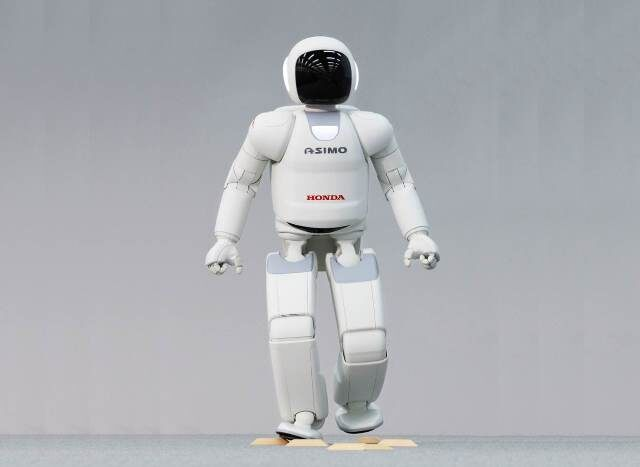
\includegraphics[width=0.8\textwidth]{figura1refbot.png}			
	\caption{ASIMO}		
	\label{img:denavit}	
	\source{HONDA}		
\end{figure}


O uso de robôs industriais como o UNIMATE tem como principal reflexo a automatização da produção, aumentando, portanto, a quantidade de produtos gerados em dado período de tempo. Outro fator que pode ser relacionado ao uso de robôs em linha de produção é a melhora nas condições de trabalho do ser humano, por meio da redução de atividades perigosas ou insalubres \cite{bouteille}.
O controle de sistemas robóticos, com o passar dos anos, vem se tornando mais complexo e especializado, porém pode ser simplificado para um controle de malha fechada, que pode ser visto na Figura 02.

\begin{figure}[h!]												
	\centering												
	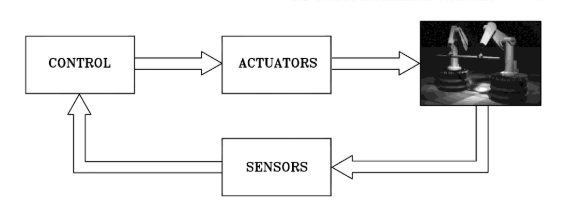
\includegraphics[width=1.0\textwidth]{figura2refbot.png}			
	\caption{Componentes e controle de robôs}		
	\label{img:denavit}	
	\source{\cite{siciliano2010}}		
\end{figure}

Percebe-se, a partir da Figura 02 que, em sistemas robóticos, existem atuadores e sensores. Atuadores podem ser citados como sistemas que possuem a capacidade de exercer atuação mecânica para o robô, como o exemplo dos servo-motores. Sensores são transmissores que recebem determinado dado e emitem sinais analógicos ou digitais para o computador central, possibilitando o controle de um sistema robótico. 





\subsection{Percepção}\label{sec:perception}
Segundo \cite{lent}, para a neurociência, a percepção refere-se à capacidade de associar automaticamente as informações sensoriais à memória e à cognição de tal maneira a gerar conceitos sobre o mundo e orientar os comportamentos. Comparativamente, o robô associa os dados “sensoriais” obtidos através dos sensores aos controladores para que possam ser processados e interpretados, dando assim, a capacidade de percepção aos robôs. 

Atualmente, existem diversos sensores que são utilizados, dentre eles: LIDAR, câmeras, IMU, sensores de temperatura, umidade etc. A capacidade de conectar uma ação a partir da percepção de mundo é tarefa do controle, o qual pode emitir comandos de execução para os atuadores a partir das leituras dos sensores. Um exemplo prático disso é o ser humano: quando uma pessoa bate o dedinho do pé, instantaneamente, as terminações nervosas (sensores) emitirão sinais ao cérebro (controle), que por sua vez, emitirá um sinal para os músculos (atuadores) se moverem a fim de interromper a sensação dolorosa.    

A visão computacional é a tentativa de simular a visão biológica, o que se torna em um assunto extremamente complexo. \cite{jahne} escreve que pode-se comparar as funcionalidades básicas dos dois tipo de visão, que são:

\begin{itemize}
	\item Fonte de radiação: sem a emissão de radiação nada pode ser observado ou processado;
	
	\item Câmera: dispositivo que captura a radiação emitida;
	
	\item Sensor: dispositivo que converte a radiação capturada em sinal apropriado para o processamento;
	
    \item Unidade de processamento: dispositivo que processa os sinais convertidos extraindo informações adequadas para a medição do objeto e categorizá-las em classes;
    \item Atuadores: utilização as informações processadas para realizar alguma ação.
    
\end{itemize}

Após esclarecidas as principais funções básicas da visão, também é necessário entender que a visão computacional não é somente o processamento de imagens. O processamento de imagens recebe uma imagem como entrada, e como saída tem-se um conjunto de valores numéricos que podem ou não formar outra imagem. Já a visão computacional é a busca de simular a visão humana, em que a entrada é uma imagem, e a saída é a interpretação dela. 

\cite{gonzalez} escrevem que não existe uma fronteira bem definida entre o processamento de imagens e a visão computacional. Porém é possível dividir o caminho entre o processamento de imagem e a visão computacional em três partes: nível baixo, nível médio e nível alto. O nível baixo é de processos primitivos, como pré-processamento de imagem para redução de ruídos, aprimoramento de contraste e nitidez da imagem. Já o nível médio é caracterizado por processos que têm como entrada imagens, mas a saída do processamento são atributos extraídos da imagem, como arestas, contornos e identificação de objetos. O nível alto trata-se dos processos que interpretam um conjunto de objetos reconhecidos na imagem, desta maneira, realizando funções cognitivas que geralmente são associadas à visão biológica.

As aplicações da visão computacional são bastante amplas, e pode ser usada desde para o aumento da produtividade de uma linha de produção através da rápida inspeção, até para que robôs possam compreender seus arredores. Um bom exemplo da utilização da visão computacional é nos veículos autônomos, em câmeras, como podem ser vistos na Figura 03, são utilizadas em conjunto com outros tipos de sensores para possibilitar que o automóvel utilize o piloto automático. 

\begin{figure}[h!]												
	\centering												
	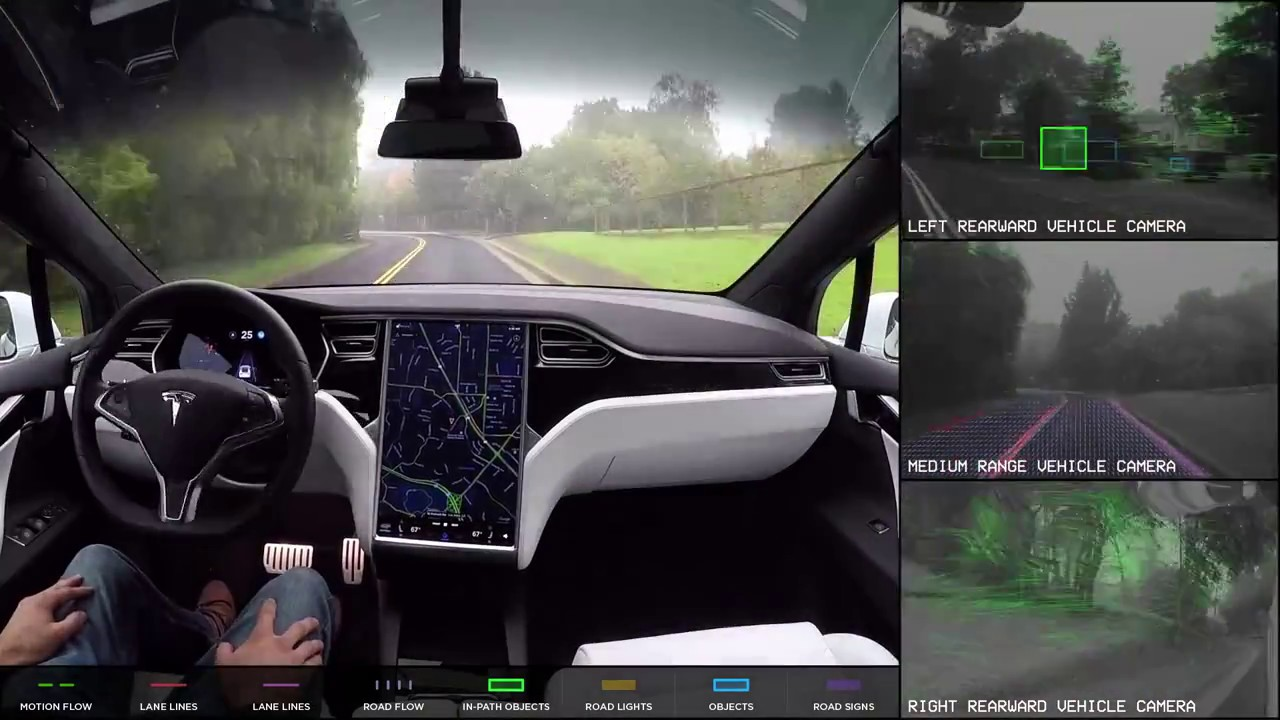
\includegraphics[width=1.0\textwidth]{figura3refbot.png}			
	\caption{Visão da câmera - Piloto automático}		
	\label{img:denavit}	
	\source{Tesla}		
\end{figure}

Para que um robô móvel seja autônomo, deve ser capaz de perceber o ambiente à sua volta para que assim possa decidir sobre qual a melhor ação a ser tomada e realizá-la com o menor erro possível. Desta maneira, um das funções fundamentais do robô a fim de alcançar seu objetivo, tanto em ambientes externos quanto em ambientes internos, é a aquisição de informações do ambiente em que está localizado através da construção de mapas do local. Segundo \cite{murphy} os mapas utilizados para navegação dos robôs podem ser classificados, de acordo com sua estrutura, em dois tipos:

\begin{itemize}
	\item Topológicos: modelo que representa o ambiente por meio de conexão entre pontos de referência. A representação pode ser feita por meio de grafos onde os vértices representam os locais e as arestas representam o caminho entre os locais. Porém esse tipo de representação é pobre em detalhes do ambiente físico;
	
	\item Métricos: modelo que representa o ambiente físico em detalhes. A representação do ambiente é normalmente feita através de um plano dividido em células de tamanhos iguais, que também é chamada de grade. Desta maneira, cada célula representa uma parte do espaço físico.
\end{itemize}

\subsection{Áreas de Atuação}\label{sec:atuation}
Com a união dos sensores, atuadores e um controle lógico, o ser humano tem a possibilidade de criar robôs para uma infinidade de áreas de atuações. \cite{siciliano2016} descreve algumas das possíveis áreas em que a robótica pode atuar, como por exemplo:

\begin{itemize}
	\item Industrial;
	
	\item Subaquática;
	
	\item Aéreo;
	
	\item Espacial;
	
	\item Educação.
\end{itemize}

Na área industrial, como visto anteriormente, foi o pontapé para o desenvolvimento da robótica devido a necessidade do aumento de produtividade das grandes empresas. E nesta área a robótica pode atuar em alguns setores, como por exemplo:

\begin{itemize}
	\item Soldagem: com a necessidade de uma mão de obra muito especializada devido a grande chance de pequenas imperfeições, que podem levar a grandes consequências, foi introduzido a robótica no processo de soldagem industrial para garantir a repetibilidade do processo;
	
	\item Transferência/posicionamento de material: da mesma maneira que a soldagem, a robótica foi introduzida para reduzir os danos ocupacionais aos colaboradores causados pelos movimentos repetitivos e levantamento de peso excessivo. Assim como para assegurar a repetibilidade do processo;
	
	\item Pintura: motivado pelas condições perigosas de trabalho, a robótica foi inserida neste contexto para reduzir os impactos das tintas na saúde dos operadores e também para garantir a repetibilidade e a eficiência do processo;
	
	\item Usinagem: utilizado devido a sua grande precisão, podem ser utilizado nos mais diversos campos da usinagem bastando apenas providenciar a ferramenta adequada.
\end{itemize}

“Os oceanos cobrem cerca de 2/3 da superfície da terra e tem sido crítico para o bem-estar dos seres humanos por toda a história. Atualmente, os mares são uma importante fonte de alimento e outros recursos, como petróleo e gás.” \cite{siciliano2016}. Como destacado pelo autor, os mares e oceanos são peças fundamentais para o desenvolvimento humano ao longo do tempo. No início da exploração subaquática o ser humano contava apenas com mergulhos e veículos submersíveis tripulados. 

Porém, existe a necessidade de explorar regiões que expõem a segurança dos seres humanos, e por conta desta necessidade foram desenvolvidos robôs, seja autônomos ou remotamente operados,  para que assim fosse possível suprir tais necessidades. Atualmente os robôs subaquáticos atuam em três áreas: comercial, científica e militar. Dentre as áreas de atuação, as atividades mais praticadas são a inspeção (equipamentos, tubulações, terreno), instalação e manutenção (equipamentos e tubulações), pesquisa e coleta de objetos.

O grande índice de fatalidades com aeronaves operadas por seres humanos levou os engenheiros a desenvolver máquinas voadoras capazes de ser operadas sem a presença de humanos \cite{siciliano2016}. Com isto os robôs têm grande papel no desenvolvimento de aeronaves não tripuladas. Algumas das aplicações dos robôs nesta área são:

\begin{itemize}
	\item Observação aérea: podem ser usados tanto para uso civil quanto para militar, podem fazer as seguintes ações: mapeamento de terreno, pesquisas ambientais, monitoramento de plantações, filmagens, identificação de alvos;
	
	\item Entrega de carga: utilizados para entrega de carga em locais de difícil acesso às pessoas. Muito utilizados também para fazer a aplicação de agrotóxicos em plantações. Utilizado também pelo os militares para a entrega de mísseis. 
\end{itemize}

Os robôs são excelentes soluções para o ambiente extremamente perigoso que é o espaço. Segundo a \cite{nasa_2017}, os robôs são utilizados por diversos motivos, o mais importante deles é a segurança para os seres humanos, uma vez que robô podem ser dispensados. Outro motivo é o custo, enviar robôs para o espaço é mais barato que enviar humanos, pois eles não têm as necessidades que os seres humanos têm. Segundo \cite{esa_2014} os robôs espaciais tem duas principais aplicações: 

\begin{itemize}
	\item Orbital: usado basicamente para a construção, operação e manutenção da Estação Espacial Internacional (ISS) ou de satélites que orbitam o planeta, através de braços robóticos;
	
	\item Exploração planetária: viagens longas e perigosas impulsionaram o desenvolvimento de robôs capazes de vasculharem a superfície de planetas ou corpos celestes. Existem uma variedade de robôs com este propósito, como por exemplo rovers e hoppers, penetrômetros e toupeira robótica, balões, dirigíveis e aviões. 
\end{itemize}

Na educação, os robôs acabam sendo poderosas ferramentas de aprendizado, cada vez mais inseridos no mercado. \cite{siciliano2016} escreve que os robôs, no contexto educacional, possuem três papéis principais. O primeiro é o robô como um projeto de linguagem de programação, que se utiliza um exemplo contextualizado para motivar os estudantes se aprofundarem no assunto. O segundo papel é o robô como foco de aprendizado, em que se utiliza um robô físico para ensinar os mais diversos assuntos técnicos durante a construção de um robô. O terceiro e último papel é o robô como colaborador de aprendizado, em que o estudante não está projetando um robô, mas tendo um robô de alto nível como companheiro de aprendizado. Com esses papéis, a robótica consegue desenvolver o estudante em alguns pontos: 

\begin{itemize}
	\item No interesse na ciência e engenharia;
	
	\item No trabalho em equipe;
	
	\item Na resolução de problemas 
\end{itemize}



